%% Author: Daniel Kaplan
%% Subject: Distributions (density plots)




\providecommand{\HCode}[1]{#1} % dummy, just in case it's PDFlatex
\HCode{<link rel="stylesheet" href="fixSweave.css" type="text/css"
  media="screen" />}
\HCode{<link rel="stylesheet" href="http://dl.dropbox.com/u/5098197/Math135/RGuide/fixSweave.css" type="text/css"
 media="screen" />}


The plot purports to show the density of a distribution of data.  If this is
true, the fraction of the data that falls between any two values on
the $x$ axis should be the area under the curve between those two
values.


\centerline{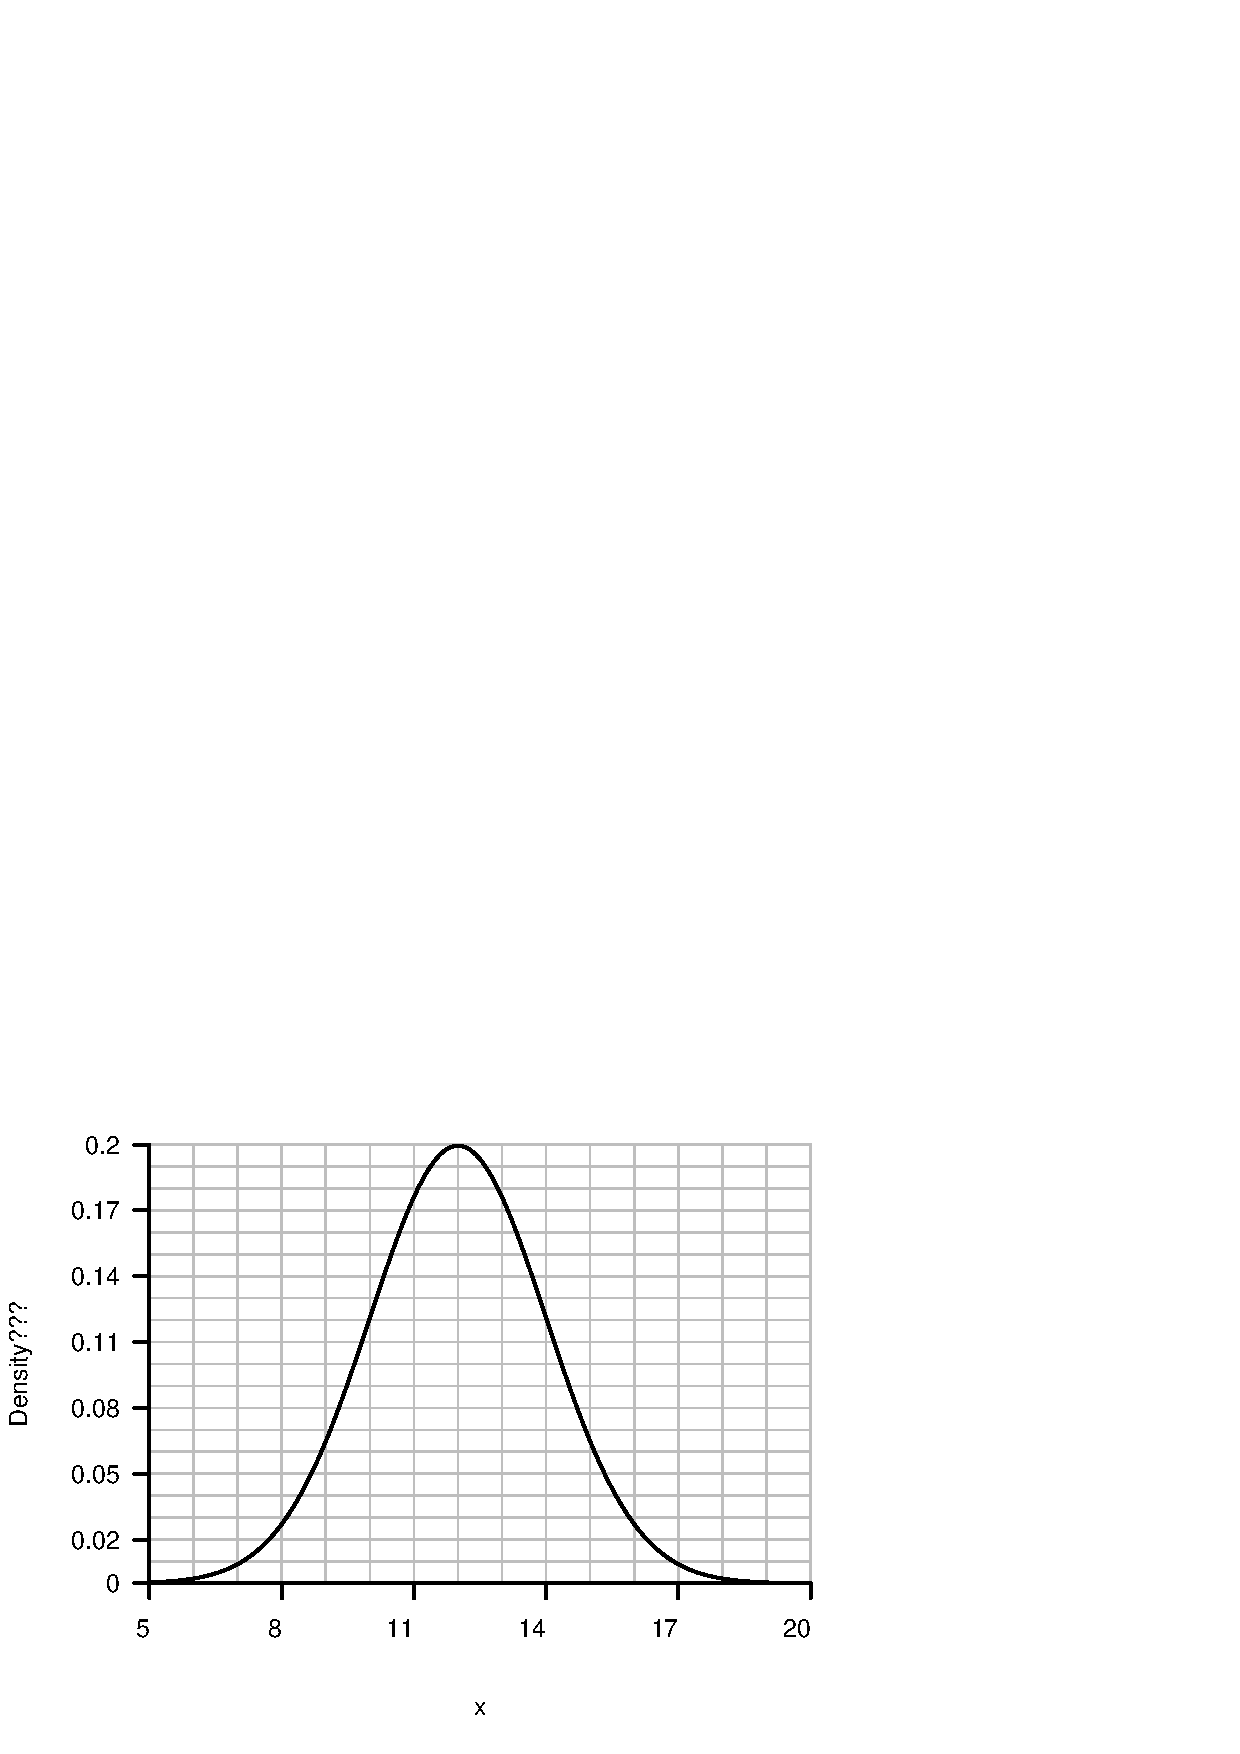
\includegraphics[width=3.5in]{Figures/B106-plot1}}

Answer the following questions. In doing so, keep in mind that the area of each
little box on the graph paper has been arranged to be $0.01$, so you
can calculate the area by counting boxes.  You don't need to be too
fanatical about dealing with boxes where only a portion in under the
curve; just eyeball things and estimate.

\begin{enumerate}[(a)]
\item The total area under a density curve should be 1.
  Assuming that the density curve has height zero outside of the area
  of the plot, is the area under the entire curve consistent with
  this?
\SelectSetHoriz{yes}{yes,no}
%\begin{MultipleChoice}
%\correct{yes}
%\wrong{no}
%\end{MultipleChoice}

\item What fraction of the data falls in the range $12 \leq x \leq
  14$?

\begin{MultipleChoice}
\wrong{14\%}
\wrong{22\%}
\correct{34\%}
\wrong{56\%}
\wrong{Can't tell from this graph.}
\end{MultipleChoice}

\item What fraction of the data falls in the range $14 \leq x \leq
  16$?

\begin{MultipleChoice}
\correct{14\%}
\wrong{22\%}
\wrong{34\%}
\wrong{56\%}
\wrong{Can't tell from this graph.}
\end{MultipleChoice}

\item What fraction of the data has $x \geq 16$?

\begin{MultipleChoice}
\wrong{1\%}
\correct{2\%}
\wrong{5\%}
\wrong{10\%}
\wrong{Can't tell from this graph.}
\end{MultipleChoice}


\item What is the width of the 95\% coverage interval.  (Note: The
  coverage interval itself has top and bottom ends.  This problem asks
  for the spacing between the two ends.)
\begin{MultipleChoice}
\wrong{2}
\wrong{4}
\correct{8}
\wrong{12}
\wrong{Can't tell from this graph.}
\end{MultipleChoice}

\end{enumerate}

